\chapter{Implementierung}
\label{chap6}

In diesem Kapitel soll die konkrete Implementierung der im vorangegangen Kapitel gezeigten Architektur detailliert erklärt werden. Für die Implementierung wird
als Grundlage die von \textcite{dm-cache} entwickelte Implementierung genutzt. Die Funktionsweise und wichtige Implementierungsdetails werden in Abschnitt
\ref{chap6:dm-cache} dargestellt. Da die Implementierung jedoch nicht die für diese Arbeit geforderten Eigenschaften erfüllt, wurden mehrere Änderungen und
Erweiterungen vorgenommen. Zunächst wurden die Debugmöglichkeiten erweitert. Dies wird in Abschnitt \ref{chap6:debug} genauer beschrieben. Des Weiteren wird die
Implementierung des oben beschriebenen Cache-Algorithmusin Abschnitt \ref{chap6:algo} dargestellt. Ferner wies das ursprüngliche Modul starke Defizite in Bezug
auf den Speicherverbrauch auf. Aus diesem Grund wurden hier Optimierungen vorgenommen, die in Abschnitt \ref{chap6:meta} genauer betrachtet werden. Auf Grund
dieser Änderungen und weiterer Defiztite bei der Metadatensicherung, musste auch diese verändert werden. Diese Veränderungen werden in Abschnitt
\ref{chap6:save} beschrieben. Weiterhin wurde im Rahmen dieser Arbeit auch die Nutzung des \texttt{TRIM}-Kommandos, welches in Abschnitt \ref{chap2:ssd}
vorgestellt wurde, berücksichtigt. Die Änderungen, die hierfür am Kernelmodul vorgenommen wurden, werden in Abschnitt \ref{chap6:trim} beleuchtet. Das
ursprüngliche Modul wies außerdem keinerlei Möglichkeit auf von einem gecachten Medium zu booten. Aus diesem Grund musste die Funktion auch von Grund auf neu
implementiert werden. Das Vorgehen hierbei wird abschließend in Abschnitt \ref{chap6:boot} erklärt

\section{Grundlage: dm-cache}
\label{chap6:dm-cache}

Als Grundlage für die Implementierung des Caches dient das von \citeauthor{dm-cache} entworfene Kernelmodul -- dm-cache genannt. Dieses nutzt den
\ac{DM} und entspricht bereits im Wesentlichen der in dieser Arbeit vorgeschlagenen High-Level-Architektur. In diesem Abschnitt soll die Funktionsweise dieses
Moduls genauer beleuchtet werden. Die Lebenszeit eines konkreten Caches lässt sich hierbei in drei Phasen teilen:

\subsection{Phase 1: Konstruktion}

Die erste Phase ist das Erstellen des Caches. Hierbei wird die Metadatenstruktur des Caches (vgl. Listing \ref{listing:cache1:meta} im Anhang) an sich angelegt.
Dasselbe gilt für die Metadaten der einzelnen Cacheblöcke (vgl. Listing \ref{listing:cache1:block} im Anhang). Das Erstellen geschieht durch einen Aufruf aus
der Nutzerebene, für gewöhnlich unter Zuhilfenahme der \ac{DM}-Tools. Der konkrete Befehl sieht dabei wie folgt aus, wobei beim letzten Parameter 0 für einen
Write-Through-Cache und 1 für einen Write-Back-Cache steht:

\begin{flushleft}
\hspace{0.25cm} \small \texttt{echo [Startblock] [Endblock] cache [Quellgerät] [Cachegerät] 0 [Cacheblockgröße] [Cacheblöcke] [Assoziativität] [0|1] | dmsetup
create [Name]}
\end{flushleft}

Die Konstruktorroutine nimmt dabei die Daten entgegen, fügt die Metainformationen entsprechend in die Datenstruktur ein und erzeugt somit einen neuen leeren
Cache. Es ist jedoch auch möglich, einen Cache aus einer vorangegangenen Sitzung wiederherzustellen. Der entsprechende Befehl lautet wie folgt:

\begin{flushleft}
\hspace{0.25cm} \small \texttt{echo [Startblock] [Endblock] cache [Quellgerät] [Cachegerät] 1 | dmsetup create [Name]}
\end{flushleft}

Dieser Befehl veranlasst die Konstruktorroutine, vom Ende des Cache-Blockgerätes eine gespeicherte Metadatenstruktur zu lesen, anstatt Standardwerte
zu benutzen. Diese ist durch einen Checksumme geschützt, so dass das Laden ungültiger Informationen verhindert wird. Parallel zu den Vorgängen im
dm-cache-Modul wird vom \ac{DM}-Framework ein neues Blockgerät angelegt, welches das gecachete Blockgerät repräsentiert und vom Nutzer bzw. Betriebssystem wie
jedes andere Blockgerät genutzt werden kann.

\subsection{Phase 2: Lebenszeit}

Nach der Konstruktion bzw. Rekonstruktion des Caches kann dieser mit der eigentlichen Arbeit beginnen. Dabei ist die Arbeit wie im High-Level-Blockdiagramm
vorgesehen, in zwei asynchron zueinander arbeitende Programmteile aufgeteilt.

\subsubsection{Teil I - Systemaufruf}

Der erste Programmteil wird immer aktiv, wenn auf das Blockgerät zugegriffen wird und Daten geschrieben oder gelesen werden. Dies geschieht für gewöhnlich durch
eine Dateioperation im Nutzerraum. Er arbeitet also synchron zu Systemaufrufen. Dabei wird vom \ac{DM}-Framework der \texttt{map}-Funktion eine \ac{BIO}-Anfrage
übergeben. Diese überprüft nun, ob die gewünschten Blöcke im Cache vorliegen und sich nicht gerade in der Bearbeitung durch den Kernelthread im zweiten
Programmteil befinden. Falls das der Fall ist, werden das Blockgerät und die Blocknummer in der \ac{BIO}-Anfrage entsprechend angepasst und durch den
entsprechenden Rückgabewert der \texttt{map}-Funktion dem \ac{DM}-Framework die Fertigstellung der \ac{BIO}-Manipulation mitgeteilt. Das \ac{DM}-Framework leitet
sodann die Anfrage an das entsprechende Gerät weiter und schließt die Anfrage ab. Sollte der Cacheblock gerade in Bearbeitung durch den Kernelthread sein, wird
die Anfrage in einer Liste in den Metadaten des Blockes vermerkt und dem Framework mitgeteilt, so dass das Modul die weitere Verarbeitung veranlassen wird.
Sollte der entsprechende Block nicht im Cache vorrätig sein, wird ein geeigneter Cacheblock nach dem \ac{LRU}-Algorithmus gesucht, um die Daten einzulagern. Sollte kein
geeigneter Block gefunden werden, was immer dann der Fall ist, wenn alle Blöcke des Sets, in dem die entsprechenden Daten eingelagert werden müssten, in
Bearbeitung durch den zweiten Programmteil sind, wird die Anfrage analog zum Vorgehen von oben auf das Quellgerät umgeleitet. Beim Auffinden eines passenden
Blockes könnte dieser bei einem Writh-Through-Cache verändert worden sein. Sollte dies der Fall sein, wird das Zurückschreiben des Blockes veranlasst und weiter
vorgegangen, wie gerade beschrieben. Anderenfalls wird dieser markiert, dass er in Bearbeitung durch den Kernelthread ist und der \ac{BIO}-Auftrag in die
Auftragsliste des zweiten Programmteils eingefügt. Dieser wird dabei in eine entsprechende Datenstruktur \ref{listing:cache1:job} verpackt, die neben der
Referenz auf die \ac{BIO}-Struktur z.B. eine Referenz auf die Metadaten des Caches und den zu nutzenden Cacheblock hat.

\subsubsection{Teil II - Kernelthread}

Der zweite Programmteil arbeitet asynchron in einem Kernelthread und ist, wie im High-Level-Blockdiagramm zu sehen, für das Ein- und Auslagern von Cacheblöcken
zuständig. Die Aufträge werden der Reihe nach aus der Auftragsliste entnommen. Sollte es sich um eine lesende Anfrage handeln, werden zunächst die Daten vom
Quellgerät in den Speicher kopiert. Dies passiert wiederum asynchron. Nach Abschluss des Vorgangs wird durch Aufruf der zuvor übergebenen Callbackmethode das
weitere Vorgehen in Gang gesetzt. Zunächst wird dem Kernel mitgeteilt, dass die \ac{BIO}-Anfrage abgeschlossen ist, so dass der anfragende Programmfluss
fortgesetzt werden kann. Anschließend werden die Daten wiederum asynchron auf das Cachegerät geschrieben. Nach dem erneuten Aufrufen der Callbackmethode wird abschließend in
dem Metadaten des Cachesblockes vermerkt, dass der betreffenden Cacheblock nicht länger in Bearbeitung ist.

\subsection{Phase 3: Destruktion}

In der dritten und letzten Phase werden zunächst die als \texttt{dirty} markierten Blöcke auf das Quellegerät zurückgeschrieben. Anschließend werden die
Metadaten des Caches an das Ende des Cachegerätes geschrieben. Hierbei werden lediglich die Blocknummern des gecachten Gerätes gespeichert, zu dem der jeweilige
Cacheblock gehört, jedoch nicht der Zeitstempel der logischen Uhr. Die Destruktion kann wiederum unter Zuhilfenahme der \ac{DM}-Tools vom Nutzer durch folgenden
Befehl veranlasst werden:

\begin{flushleft}
\hspace{0.25cm} \small \texttt{dmsetup remove [Name]}
\end{flushleft}

Parallel hierzu entfernt das \ac{DM}-Framework das logische Blockgerät, welches das gecachete Gerät repräsentiert.

\section{Debuginterface}
\label{chap6:debug}

Die gegebene Implementierung des Caches bietet leider nur unzureichende Möglichkeiten der Fehlersuche. Es wurden von den Autoren lediglich Kernellog-Nachrichten
als Debugmöglichkeit vorgesehen. Da es aber in einem Cache mehrere Millionen Cacheblöcke und noch mehr Zugriffe während eines Testlaufes geben kann, sind diese
nur bedingt geeignet. Zum einen werden die Lognachrichten in sehr kurzen Abständen ausgegeben, so dass ein Log-Daemon gar nicht in der Lage ist, alle Nachrichten
zu verarbeiten. Zum anderen kann die Datenmenge der Logmeldungen schnell auf mehrere hundert Megabyte anwachsen, so dass selbst der Puffer für
Kernellog-Nachrichten ältere Einträge fallen lassen muss. Aus diesem Grund wurden zwei weitere Debugmöglichkeiten implementiert:

\subsection{\texttt{message}-Funktion}

Die erste Möglichkeit eines erweiterten Debuggings liefert die \texttt{message}-Funktion des \ac{DM}-Frameworks, jedoch ist sie nicht darauf limitiert. Die
Funktion dient dazu, Nachrichten an eine bestimmte Instanz eines \ac{DM}-Geräts zu schicken. Diese kann dazu genutzt werden, Einstellungen zur Laufzeit
vorzunehmen bzw. zu verändern. Der Zugang aus dem Nutzerraum ist wiederum mit den \ac{DM}-Tools unter Verwendung folgenden Befehls möglich:

\begin{flushleft}
\hspace{0.25cm} \small \texttt{dmsetup message [Name] [Blocknummer] [Funktionsnummer] $\{$Argumente$\}$}
\end{flushleft}

Im Rahmen dieser Arbeit wurde zunächst die \texttt{message}-Funktion dahingehend implementiert, dass sie unter anderem weitere Debugmöglichkeiten bietet. Im
weiteren Verlauf wurde die \texttt{message}-Funktion so erweitert, dass bestimmte Cacheparameter zur Laufzeit angepasst werden können. Die konkret
implementierten Funktionen sind in Tabelle \ref{table:message} aufgeführt.

\begin{table}[H]\centering
	\newcolumntype{C}[1]{>{\centering\arraybackslash}m{#1}}
  \caption{Funktionen des \texttt{message}-Interfaces}\vspace{0.25cm}
	\begin{tabular}{l|l|l}
	\multicolumn{1}{C{1.9cm}|}{\textbf{Funktions-}\textbf{nummer}} & \multicolumn{1}{C{1.4cm}|}{\textbf{Argu-}\textbf{mente}} &
	\multicolumn{1}{c}{\textbf{Funktion}} \\ \hline \hline \multicolumn{3}{c}{\textbf{Laufzeitfunktionen}} \\ \hline \hline
	0 & -- & Zurückschreiben geänderter Blöcke Ein-/Ausschalten (toggle) \\ \hline
	\multicolumn{3}{c}{\textbf{Debugfunktionen}} \\ \hline \hline
	1 & -- & alle Cacheblock-Metadaten ausgeben \\ \hline
	2 & [Set] & Cacheblock-Metadaten des übergebenen Sets ausgeben \\ \hline
	3 & [Block] & Ausgabe des Sets, in das der Block fällt\\ \hline
	4 & -- & Ausgabe der Anzahl der Cacheblöcke in jedem Zustand\\ \hline
	5 & -- & Zurücksetzen der Statistik \\ \hline
	6 & -- & die Konsistenz des Caches prüfen\\ \hline
	\end{tabular}
	\label{table:message}
\end{table}

\subsection{\texttt{debugfs}-Interface und Visualizer}

Das \texttt{debugfs}-Dateisystem wurde entworfen, um Informationen zwischen einem Kernelmodul und dem Nutzerraum unter Zuhilfenahme des Dateisystems
auszutauschen. Die genaue Funktionsweise wird bei \cite{debugfs} erläutert und soll hier nicht näher diskutiert werden.

Das Cachemodul wurde um eine \texttt{debugfs}-Schnittstelle erweitert, um die Metadaten des Caches und der Cacheblöcke auf einfache Weise in den Nutzerraum zu
übertragen. Dies ist insbesondere bei den Metadaten der Cacheblöcke nur in binärer Form effizient möglich, da die Datenmenge auf Grund der Anzahl der Blöcke
ansonsten zu groß wäre.

Weil die Metadaten zunächst nur in binärer Form vorliegen, musste ein Weg gefunden werden, diese auszuwerten. Auf Grund der Menge der Informationen bietet sich
hierfür eine Visualisierung an, die die Daten so aufbereitet, dass sie übersichtlich bleiben. Da jedoch die Auswertung wegen der Datenmenge rechenintensiv ist,
wurde es vom Testrechner auf den Entwicklungsrechner verlagert. Hierfür werden die Daten zwischen Test- und Entwicklungsrechner per Ethernet ausgetauscht. Der
Sachverhalt ist in Abbildung \ref{img:debug1} dargestellt:

\begin{figure}[H]\centering
    \includetikz{figures/chapter6/debug1}%
    \caption[Verbindungspfad zwischen Cache-Modul und Visualizer]{Verbindungspfad zwischen Cache-Modul und Visualizer}
    \label{img:debug1}
\end{figure}

Der Visualizer wertet auf dem Entwicklungsrechner die Daten aus und stellt sie grafisch dar. Dabei werden die Cacheblöcke als farbige Quadrate dargestellt. Die
Farbe gibt Auskunft über den Zustand des jeweiligen Cacheblocks, wodurch schnell ein Überblick über die Zustände vieler Cacheblöcke verschafft werden kann.
Durch Klicken auf einen Block können schließlich genauere Informationen über diesen erhalten werden. Die Oberfläche des Visualizers ist in Abbildung \ref{img:debug2} zu sehen.

\begin{figure}[H]\centering
    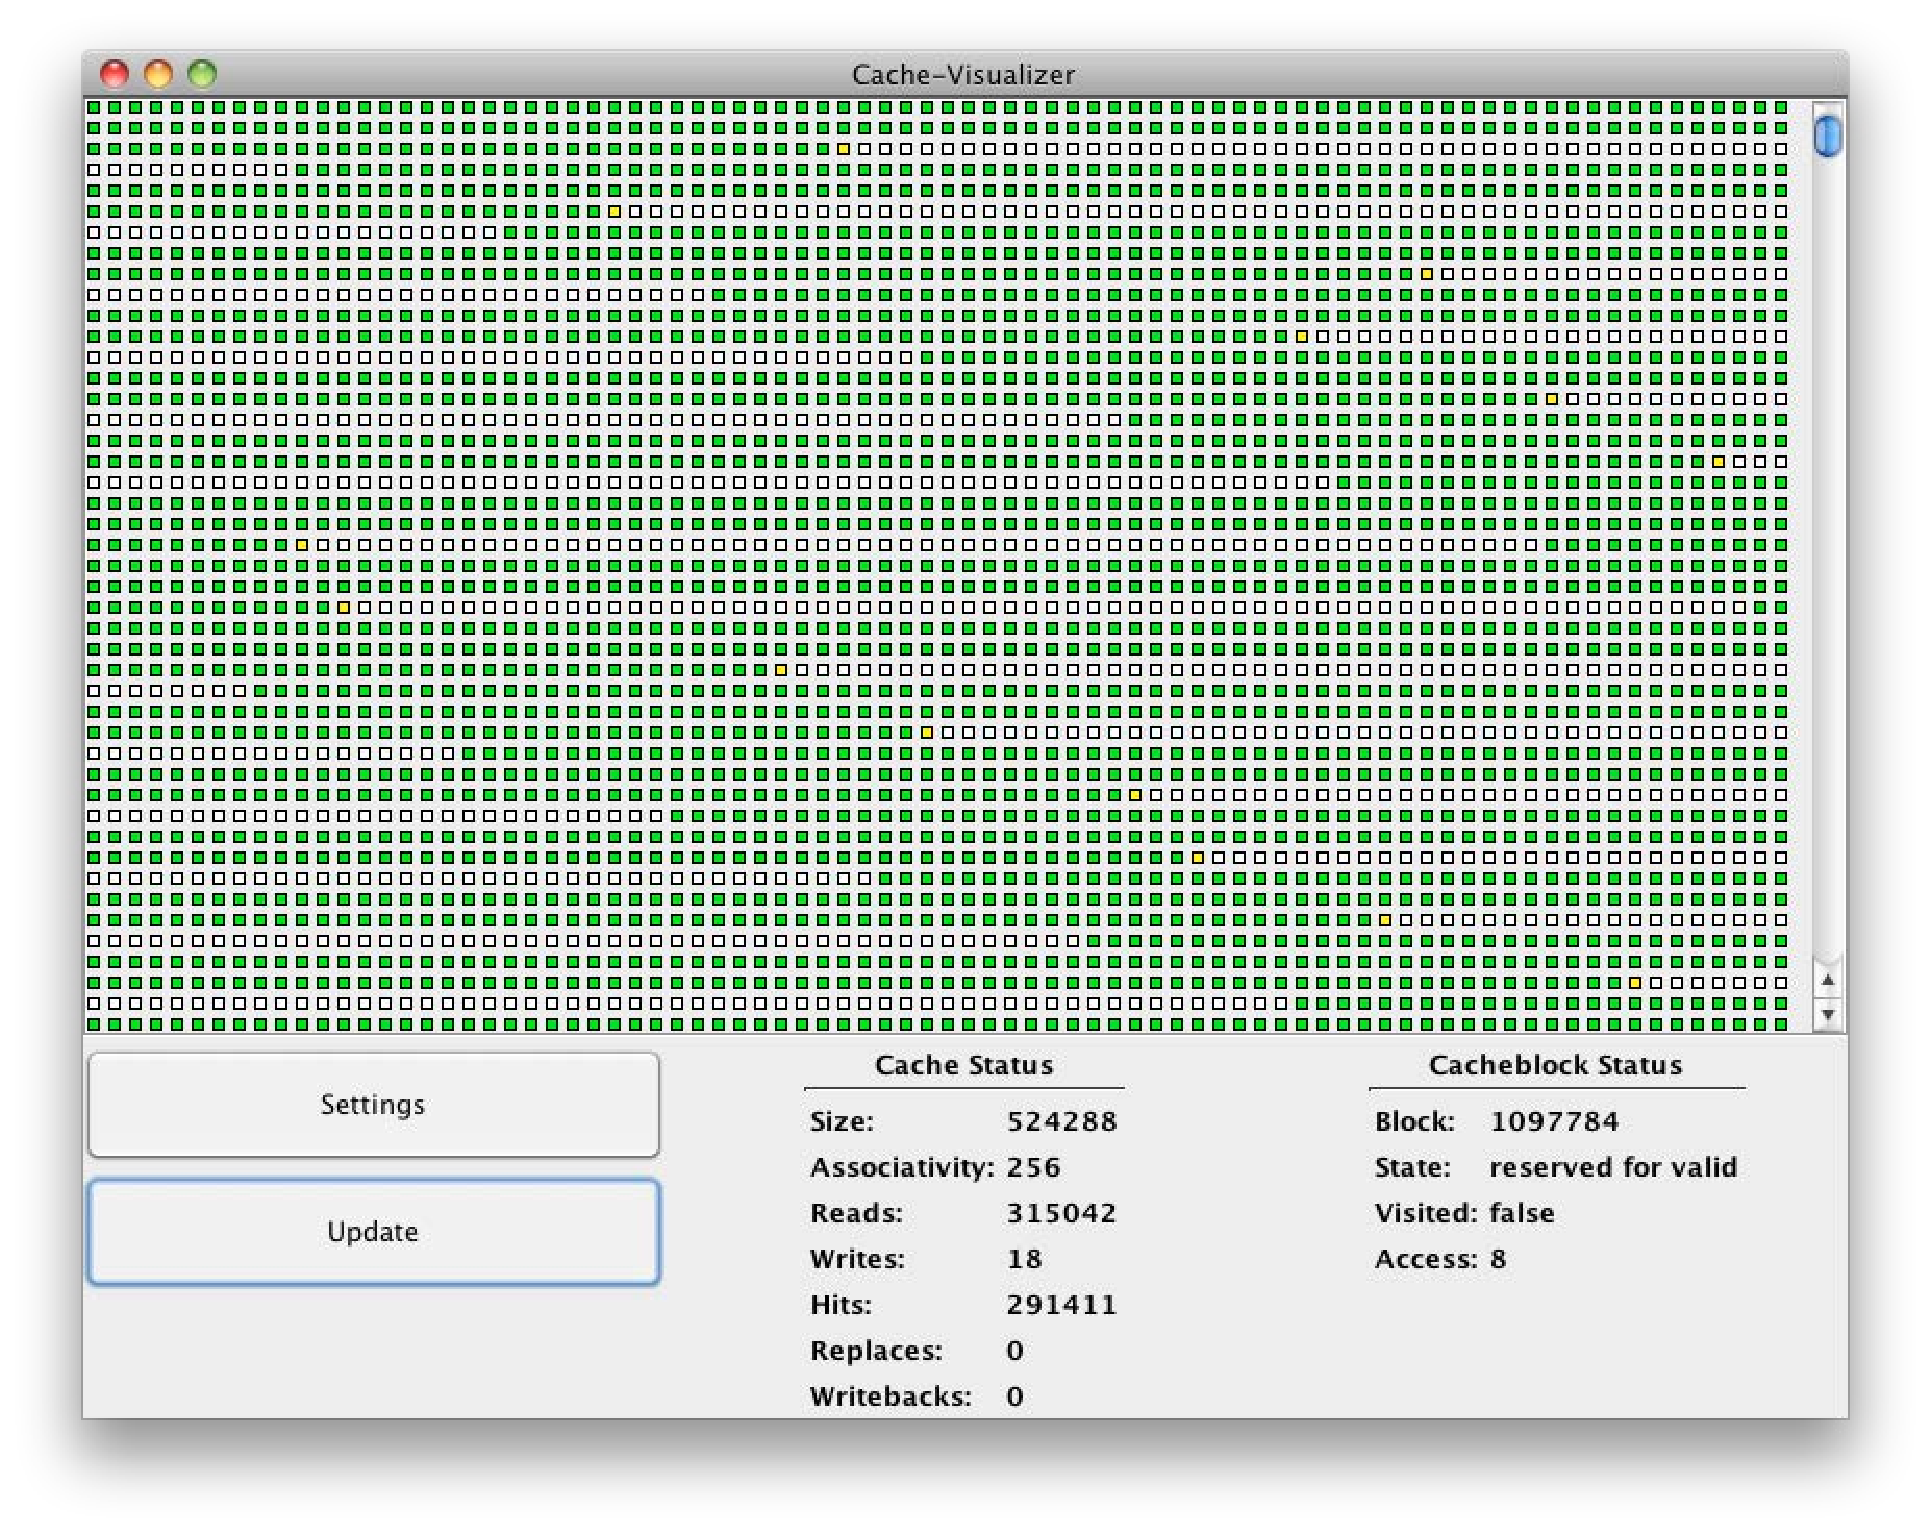
\includegraphics[scale=0.45]{figures/chapter6/screen}
    \caption[Fenster des Visualizers mit aktivem Cache]{Fenster des Visualizers mit aktivem Cache}
    \label{img:debug2}
\end{figure}
\vspace{5mm}
\section{Cache-Algorithmus}
\label{chap6:algo}

Für den in Abschnitt \ref{chap5:algo1} vorgestellten Verdrängungsalgorithmus mussten die Cacheblock-Metadatenstruktur zunächst um ein Feld für den Zähler
erweitert werden und die Cachemetadatenstruktur um einen Zähler je Set. Des Weiteren musste die Konstruktorroutine angepasst werden, so dass die Informationen
über die Werte $i$, $m$ und $s$ zur Laufzeit übergeben werden können. Außerdem wurde der Parameter für die Schreibstrategie erweitert, um das in Kapitel
\ref{chap5:algo1} beschriebene Verfahren zu unterstützen. Dies hat zur Folge, dass sich der Aufruf für das Erstellen eines Caches wie folgt erweitert:

\begin{flushleft}
\hspace{0.25cm} \small \texttt{echo [Startblock] [Endblock] cache [Quellgerät] [Cachegerät] 0 [Cacheblockgröße] [Cacheblöcke] [Assoziativität] [0|1|2]
\textbf{[s] [m] [i]} | dmsetup create [Name]}
\end{flushleft}

Weiterhin wurde die Art der Speicherung der Cacheblockzustände geändert. In der ursprünglichen Implementierung wurden Statusbits genutzt um einen Zustand zu
bestimmen. Dieses führte dazu, dass für das Speichern der Zustände mindestens\footnote{Es wurde in der konkreten Implementierung eine 16 Bit Variable benutzt.}
vier Bit benötigt wurden. Zudem machte es den Quelltext unübersichtlich, da auf den ersten Blick nicht zwingend klar war, in welchem Zustand ein Block beim
Setzen eines Bits gebracht wurde bzw. schon war. Dies ist gerade in Anbetracht der Synchronisation der beiden großen Programmteile kritisch. Aus diesem Grund
wurden die Statusinformationen auf eindeutige Zustände abgebildet und in eine leichter zu verstehende Zustandsmaschine überführt (Abbildungen \ref{img:fsm1} und
\ref{img:fsm2}). Für die bessere Verständlichkeit werden an dieser Stelle Write-Through- und Write-Back-Cache getrennt dargestellt. Die komplette
Zustandsmaschine des Caches findet sich im Anhang unter Abbildung \ref{img:fsm3}. Die Zustandsmaschine für den Write-Hybride-Cache entspricht der des
Write-Back-Caches, wobei der Zustand \texttt{Reserved for Dirty} und die Übergänge dorthin bzw. von dort abgehend entfallen.

\begin{figure}[H]\centering
	\subfigure[]{
		\includetikz[0.66]{figures/chapter6/fsm1}%
		\label{img:fsm1}
	}
	\hfill
	\subfigure[]{
		\includetikz[0.66]{figures/chapter6/fsm2}%
		\label{img:fsm2}
	}
	\caption[Zustände und Zustandsübergänge der Cacheblöcke]{Zustände und Zustandsübergänge der Cacheblöcke -- in (a) für die Write-Through-Konfiguration und in (b) für die Write-Back-Konfiguration}
\end{figure}

\section{Optimierung der Cacheblock-Metadaten}
\label{chap6:meta}

Um einen möglichst geringen Speicherverbrauch zu erreichen, mussten die Metadaten der Cacheblöcke optimiert werden. Diese enthielten in der ursprünglichen
Implementierung jeweils eine Liste, um die Anfragen aufzunehmen, die während der Bearbeitung eines Cacheblockes ankommen und nicht sofort bearbeitet werden
können. Da diese Listen von den beiden zueinander asynchron laufenden Programmteilen genutzt wurden, mussten die Zugriffe synchronisiert werden. Aus diesem Grund
gab es für jeden Cacheblock eine Schlossvariable. Dies bedeutete einen Speicherverbrauch von 38 Byte pro Cacheblock. Welche Auswirkung diese Größe auf den
Gesamtspeicherverbrauch des Caches hat wird in Abschnitt \ref{chap7:mem} ausführlich betrachtet.

Erste Tests ergaben jedoch, dass diese Listen relativ selten genutzt wurden. Aus diesem Grund wurden sie durch eine gemeinsame Liste pro Cacheblock ersetzt,
welche in den Gesamtcache-Metadaten untergebracht wurden. Dies benötigte mehrere Anpassungen im Quelltext. Zunächst wurde der Callback-Funktion für das
Zurückschreiben von Cache\-blö\-cken auf das Quellgerät lediglich eine Referenz auf den geschriebenen Cacheblock übergeben. Das war ausreichend, da der Cacheblock
alle Referenzen auf die zu verändernden Daten enthielt. Durch das Verschieben der Liste für ausstehende \ac{BIO}-Anfragen musste die übergebene Datenstruktur
angepasst werden, da diese Referenz nicht mehr in den Metadaten enthalten war. Hierfür wurden die Cacheblock-Metadaten in eine erweiterte Datenstruktur
verpackt, wie sie in Listing \ref{listing:cache2:adv_cacheblock} zu sehen ist.

\lstset{language=C,
		basicstyle=\ttfamily\scriptsize,
		backgroundcolor=\color{lightgray},
		captionpos=b, 
		tabsize=4,
		showstringspaces=false,
		keepspaces=true,
		linewidth=.85\textwidth,
		xleftmargin=.15\textwidth,
		commentstyle=\color{comment},
		keywordstyle=\bfseries\color{keyword},
		stringstyle=\color{string},
		morecomment=[s][\color{javadoc}]{/**}{*/}}

\lstinputlisting[frame=trbl,caption=Metadatenstruktur für die Übergabe an die Write-Back-Callback-Funktion, label=listing:cache2:adv_cacheblock]{listings/struct_adv_cacheblock.source}

Da es ineffizient wäre, alle \ac{BIO}-Aufträge lediglich hintereinander in eine Liste einzufügen und beim Callback des Kopiervorgangs die zu einem Cacheblock
gehörenden  \acp{BIO} herauszusuchen, sind die Einträge in der neuen Auftragsliste nach Cache\-blö\-cken sortiert. Aus dieser Anforderung ergab sich die
Listenform in Listing \ref{listing:cache2:queue}. Um nun nicht bei jedem Callback die Liste durchsuchen zu müssen, auch wenn keine ausstehenden Anfragen für einen
Cacheblock vorliegen, wurde ein zusätzliches Statusbit in die Cacheblock-Metadaten eingefügt. Dieses zeigt an, ob Aufträge für den Cacheblock vorliegen oder
nicht. Wenn dies nicht der Fall ist, braucht die Liste nicht durchsucht zu werden.

\lstinputlisting[frame=trbl,caption=Listenstruktur für ausstehende BIO-Aufträge, label=listing:cache2:queue]{listings/struct_queued_bios.source}

Durch die vorherigen Änderungen war es möglich, die Cacheblock-Metadatenstruktur im Hinblick auf den
Speicherverbrauch zu optimieren. Mit der bisher verwendeten 64-Bit langen Blocknummervariablen lassen sich bis zu $2^{64}$ Blöcke bzw. 16PB bei einer Blockgröße
von 512 Byte adressieren. Da diese Datenmenge in absehbarer Zeit nicht auf einem Gerät zur Verfügung stehen wird, wurden einige Bits dieser Statusvariablen für
die zusätzlichen Informationen verwendet. Die genaue Aufteilung der 64-Bit Variablen ist in Abbildung \ref{img:block} zu sehen. Die verbleibenden 56-Bit reichen
jedoch immer noch für 64EB Daten zu 512 Byte Blöcken. Da heutige Festplatten eine Kapazität von maximal 2TB aufweisen, ist es unwahrscheinlich, dass das Modul an
seine Grenzen stößt. Das Modul kann jedoch bei Bedarf auf größere Blocknummern umgestellt werden. So ist es in Zukunft möglich, größere Blockgeräte
zu unterstützen. Dabei dürfte auch der wachsende Speicherverbrauch unkritisch sein, da anzunehmen ist, dass die Größe des Arbeitsspeichers parallel zur
Festplattenkapazität wächst.

\begin{figure}[H]\centering
	  \includetikz{figures/chapter6/cacheblockmeta}%
    \caption[Aufbau der Cacheblock-Metadaten für das neue Kernelmodul]{Aufbau der Cacheblock-Metadaten für das neue Kernelmodul}
    \label{img:block}
\end{figure}

Die konkrete Implementierung der Datenstruktur (Listing \ref{listing:cache2:block}) zeigt, dass diese leicht erweiterbar ist. Der Zähler für den
Ersetzungsalgorithmus ist mit einer Länge von vier Bit an dieser Stelle sehr willkürlich gewählt und könnte auf Kosten der maximal addressierbaren Blöcke
problemlos erweitert werden, sollte sich dies zu einem späteren Zeitpunkt als Vorteilhaft erweisen.

\lstinputlisting[frame=trbl,caption=Optimiert Datenstruktur für Cacheblock-Metainformationen, label=listing:cache2:block]{listings/struct_cacheblock2.source}

\section{Anpassung der Metadatensicherung}
\label{chap6:save}

Auf Grund der Änderung der Cacheblock-Metadatenstruktur musste auch die Sicherung dieser Daten angepasst werden. Die Daten werden prinzipiell am Ende des
Cachegeräts gespeichert. Somit muss dieses nicht nur so groß sein wie der Cache, sondern um die Größe der Metadaten größer. Die ursprüngliche Implementierung
sorgte dafür, dass vor dem Speichern der Metadaten alle Cacheblöcke, die sich im \texttt{dirty} Zustand befanden, auf das Quellgerät zurückgeschrieben wurden.
Aus diesem Grund befanden sich beim Sichern alle Cachblöcke im \texttt{valid} oder \texttt{invalid} Zustand. Beim Sichern wurde lediglich der Status der
Cacheblöcke und die bei der Konstruktion übergebenen Parameter gesichert. Die logischen Zeitstempel wurden verworfen. Des Weiteren wurden die Informationen in
einem Puffer kopiert, da nur Datenblöcke mit einer Größe, die ein Vielfaches von 512 Byte sind, auf das Blockgerät geschrieben werden können.

Dieses Vorgehen wurde dahingehend geändert, dass nun sämtliche Metadaten der Cache\-blö\-cken gesichert werden.  Zusätzlich mussten im Gegensatz zu oben die Zeiger
für das Iterieren über den Sets gesichert werden. Es wird außerdem auf die Nutzung eines Puffers verzichtet, was das Schreiben und Wiederherstellen der Daten ein
wenig beschleunigt, da auf Kopiervorgänge im Speicher verzichtet werden kann. Dies bedeutet zwar ggf. einen Verschnitt, da der Speicherblock für die Metadaten
auf ein Vielfaches von 512 Byte aufgerundet werden muss. Da es jedoch nur zwei Speicherblöcke gibt (Cacheblock-Metadaten und Iterierungszeiger), kann der
Verschnitt nicht mehr als ein Kilobyte betragen.

Es wurde des Weiteren die Fehlererkennung bei der Wiederherstellung des Caches verbessert. Bei der ursprünglichen Implementierung wurden die gesicherten
Metadaten lediglich gelesen und wiederhergestellt. Dies führte dazu, dass bei einem Absturz des Systems und anschließendem Neustart die veralteten Metadaten
wiederhergestellt wurden. Dadurch kam es zu einem inkonsistenten Cache und im ungünstigsten Fall zum Datenverlust bzw. Absturz des Systems. Aus diesem Grund
wurde die Wiederherstellung verändert in der Weise, dass der ausgelesenen Cachemetadatenblock modifiziert wurde. Es ist ein Flag eingefügt worden, welches nach dem
Auslesen geändert und verändert zurück geschrieben wird. Dadurch war es möglich zu erkennen, ob die gelesenen Metadaten zu den auf dem Cachegerät gespeicherten
Datenblöcken passen. Sollte dies nicht der Fall gewesen sein, war es weiterhin dennoch möglich den Cache neu aufzubauen, sofern es sich um einen
Write-Through-Cache handelte. Bei einem Write-Back- bzw. Write-Hybrid-Cache kann auch durch dieses Verfahren der Cache nicht wiederhergestellt oder neu aufgebaut
werden, weil durch den Systemabstrurz die Metainformationen über die Cacheblöcke verloren gegangen sind und im Nachhinein nicht mehr festgestellt werden kann,
welche Cacheblöcke ausschließlich auf dem Cacheblockgerät aktuell sind und stattdessen auf dem Quellgerät gentutz werden müssten.

\section{\texttt{TRIM} Unterstützung}
\label{chap6:trim}

Das \texttt{TRIM}-Kommando wurde bereits in Kapitel \ref{chap2:ssd} erläutert. Es wurde ausgeführt, dass eine explizite Unterstützung in das Dateisystem
eingebaut werden muss. Bei der Implementierung des Caches war es jedoch möglich, für einen bestimmten Fall diese Unterstützung auch unabhängig vom Dateisystem
anzubieten. Wie in Abbildung \ref{img:fsm1} dargestellt, existiert beim Writh-Through-Cache ein Übergang in den \texttt{invalid} Zustand. An diesem Punkt ist die
Nutzung des \texttt{TRIM}-Kommandos sinnvoll, da der Inhalt des Cacheblockes nicht mehr benötigt wird und dies somit auch dem \ac{SSD} mitgeteilt werden kann.
Deshalb wird bei der Änderung des Cacheblock-Zustandes das \texttt{TRIM}-Kommando an das \ac{SSD} übermittelt. Dieses Verhalten ist zwar per Compiler-Makro ein-
und auschaltbar, jedoch sollte es selbst bei \acp{SSD} ohne \texttt{TRIM}-Unterstüztung zu keinem Leistungsverlust führen, da der Funktionsaufruf zum Löschen
asynchron ist (siehe \cite{linux:trim}) und sofort returnieren würde.

Das \texttt{TRIM}-Kommando fand jedoch auch Anwendung bei der Erstellung des Caches. Wie ebenfalls in Kapitel \ref{chap2:ssd} angesprochen wurde, nimmt die
Leistung eines \ac{SSD} über einen längeren Nutzungszeitraum ab, da zu wenige freie Blöcke zur Verfügung stehen. Dieses Szenario könnte vielleicht bereits beim
Nauaufbau eines Caches gegeben sein. Aus diesem Grund erschien es sinnvoll, vor der Nutzung den für den Cache vorgesehenen Datenbereich mit dem
\texttt{TRIM}-Kommando zu löschen. Dies ist nicht nur dahingehend sinnvoll, dass das \ac{SSD} bereits vor der Verwendung als Cache anderweitig genutzt wurde,
sondern auch für das Szenario, dass bei jedem Bootvorgang der Cache neu erstellt wird.

\section{Bootfähigkeit des Cachemediums}
\label{chap6:boot}

Das Booten eines Linuxsystems von einem Blockgerät setzt voraus, dass dieses beim Starten des \texttt{init}-Programms zur Verfügung steht. Da das
\texttt{dm-cache}-Modul in der ursprünglichen Implementierung eine Konfiguration aus dem Nutzerraum heraus erfordert, ist diese Voraussetzung nicht gegeben. Um
nun das Booten trotzdem zu ermöglichen gibt es zwei verschiedene Möglichkeiten. Die Erste nutzt das \textit{initramfs}. Da die Erklärung der genauen
Funktionsweise des \textit{initramfs'} den Rahmen dieser Arbeit sprengen würde, wird auf \cite{initramfs} verwiesen. Durch das \textit{initramfs} ist es möglich
zunächst ein gecachetes Blockgerät aus dem Nutzerraum zu erstellen und das Wurzeldateisystem drauf umzulenken.

Die zweite Möglichkeit besteht darin, die nötige Funktionalität für das Erstellen eines \ac{DM}-Blockgeräts direkt im Kernel fest zu implementieren, so dass beim
Übergang zum \texttt{init}-Programm das gecachte Blockgerät bereits existiert. Im offiziellen Entwicklungszweig des Linux-Kernels ist die Funktion zum Erstellen
von \ac{DM}-Geräte direkt aus dem Kernel heraus nicht vorgesehen. Es existiert jedoch bei \cite{boot-patch} ein Patch, der diese Funktion in den Kernel einfügt.
Durch diesen Patch ist es möglich, dem Kernel durch den Bootloader zusätzliche Parameter zu übergeben, um ein \ac{DM}-Gerät während des Bootens zu erzeugen. Der
zusätzliche Parameter sieht dabei wie folgt aus:

\begin{flushleft}
\hspace{0.25cm} \small \texttt{dm=\dq [name] [uuid] [ro], [parameter]\dq}
\end{flushleft}

Das \ac{DM}-Gerät wird zunächst unter dem Gerätepfad \texttt{/dev/dm-*} zur Verfügung gestellt. Hierbei steht das Sternchen für eine Nummerierung, welche bei bei
null beginnt. Dem Kernel muss somit das entsprechende Gerät im \texttt{root}-Parameter übergeben werden. Bei der Nutzung von \textit{udev} wird das Gerät beim
Booten zu \texttt{/dev/mapper/[name]} umbenannt, wobei \texttt{name} dem obigen im Kernelparameter entspricht. Weiterhin steht \texttt{uuid} für den \ac{UUID} ,
den das Gerät erhalten soll. Auf die Funktionsweise des \ac{UUID} soll in dieser Arbeit nicht genauer eingegangen werden, aber es wird hierfür auf \cite{uuid}
verwiesen. Soll dem Gerät kein \ac{UUID} zugewiesen werden, ist in das Feld \texttt{none} einzutragen. Der Parameter \texttt{ro} steht für die Einstellung, ob
vom \ac{DM}-Geräte lediglich gelesen oder sowohl gelesen als auch geschrieben werden kann. Die darauf folgenden Parameter entsprechen im wesentlichen den an
\texttt{dmsetup} übergebenen Parametern zum Erstellen eines \ac{DM}-Geräts. Somit würde der Kernelparameter für ein gecachetes Blockgerät, welches unter
\texttt{/dev/mapper/cached} zur Verfügung gestellt wird, wie folgt aussehen:

\begin{flushleft}
\hspace{0.25cm} \small \texttt{dm=\dq cached none 0, [Startblock] [Endblock] cache [Quellgerät] [Cachegerät] 0 [Cacheblockgröße] [Cacheblöcke] [Assoziativität]
[0|1|2] [s] [m] [i]\dq}
\end{flushleft}

Dabei wird ein neuer Cache erstellt. Um einen bestehenden Cache wiederherzustellen, muss der Kernel-Parameter wie folgt lauten:

\begin{flushleft}
\hspace{0.25cm} \small \texttt{dm=\dq cached none 0, [Startblock] [Endblock] cache [Quellgerät] [Cachegerät] 1\dq}
\end{flushleft}

Mit dem bestehenden Patch funktionierte das Erstellen des gecachten Mediums und Booten an sich problemlos. Der Patch hatte jedoch das Defizit, dass die
Destruktionsroutine des Caches beim Herunterfahren des Systems nicht aufgerufen wurde. Ebenfalls war es nicht möglich die Destruktionsroutine aus dem Nutzerraum
während des Herunterfahrens aufzurufen, da das gecachte Gerät als Rootdateisystem eingebunden war. Dies zog einen Verlust der Metadaten nach sich und verhinderte
das erneute Booten. Somit war der Cache in diesem Zustand als Rootdateisystem nicht nutzbar. Es musste ein Weg gefunden werden, durch den beim Herunterfahren
bzw. Neustart des Systems die Metadaten gesichert werden können. Hierbei gab es wiederum zwei Möglichkeiten. Zum einen eine Erweiterung des \ac{DM}-Frameworks
und zum anderen die Erweiterung des Cachemoduls. Auf Grund der beschränkten Bearbeitungszeit wurde auf die allgemeinere Implementierung im \ac{DM} verzichtet
und statt dessen das Cachemodul entsprechend erweitert.

Zunächst musste das Cachemodul in der Art erweitert werden, dass es über das bevorstehende Herunterfahren informiert wird. Hierfür wurden Linux
\textit{Notifiers} (siehe \cite{notifiers}) genutzt. Diese ermöglichen es, im Kernel einen Funktionsaufruf zu registrieren, welcher beim Herunterfahren bzw.
Neustart des Systems ausgeführt wird. Die hierbei übergebene Funktion wurde in der Art gestaltet, dass sie über alle verbliebenen Caches iteriert und
jeweils die Destrukturfunktion aufruft. Die Erweiterung ist in Listing \ref{listing:reboot} zu sehen.

Wie in den Zeilen 7ff zu erkennen ist, bedurfte es einer Liste aller verbleibenden Caches. Hierfür musste das Kernelmodul wiederum erweitert werden, da das
\ac{DM}-Framework keine Funktionalität vorsieht, welche das Abfragen nach \ac{DM}-Geräten eines bestimmten Typs ermöglicht. Aus diesem Grund wurde die
Cachemetadatenstruktur zu einer Kernel-Liste erweitert (vgl. Zeile 7 Listing \ref{listing:cache2:meta} im Anhang). Vom Modul selbst wird nun eine Liste aller
Cachemetadatenstrukturen verwaltet. Hierbei wird beim Erstellen eines Caches die entsprechende Struktur zur Liste hinzugefügt und beim Entfernen des Caches die
Struktur ebenfalls aus der Liste entfernt. Mit dieser Liste ist es nun möglich, bei der Benachrichtigung über das Herunterfahren die Metadaten aller Caches zu
sichern.

\lstset{language=C,
		basicstyle=\ttfamily\scriptsize,
		backgroundcolor=\color{lightgray},
		captionpos=b, 
		tabsize=4,
		showstringspaces=false,
		keepspaces=true,
		linewidth=.95\textwidth,
		xleftmargin=.05\textwidth,
		commentstyle=\color{comment},
		keywordstyle=\bfseries\color{keyword},
		stringstyle=\color{string},
		morecomment=[s][\color{javadoc}]{/**}{*/}}
\lstinputlisting[frame=trbl,caption=Erweiterung für das automatische Entfernen des Caches beim Herunterfahren,label=listing:reboot]{listings/reboot.source}
